\section{Results}

For each episode, episode scores are calculated by summing up rewards of each time step. 
In \figref{fig:td3_scatter_ep_rewards} and \figref{fig:sac_scatter_ep_rewards}, a scatter plot is visualized for each model's episode scores. 
In \figref{fig:td3_std_ep_rewards} and \figref{fig:sac_std_ep_rewards}, moving average and standard deviation is visualized for each model's episode scores. 

\begin{figure}[!ht]
	\centering
	\begin{subfigure}{.49\textwidth}
		\centering
		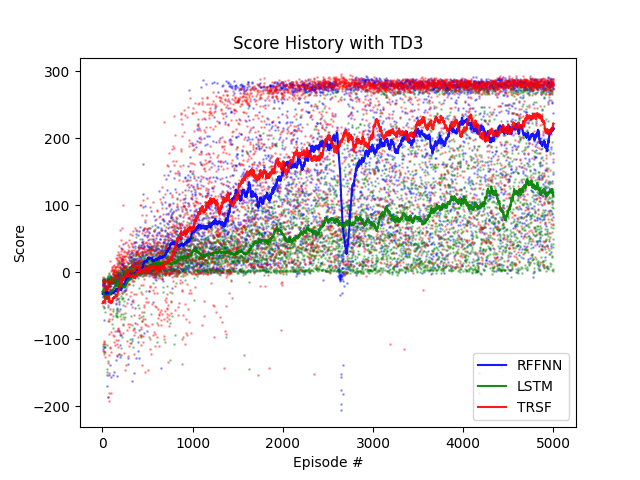
\includegraphics[width=0.99\textwidth]{figures/bipedal/SCATTER_TD3_RFFNN_LSTM_TRSF.png}
		\caption{TD3}
		\label{fig:td3_scatter_ep_rewards}
	\end{subfigure}
	\begin{subfigure}{.49\textwidth}
		\centering
		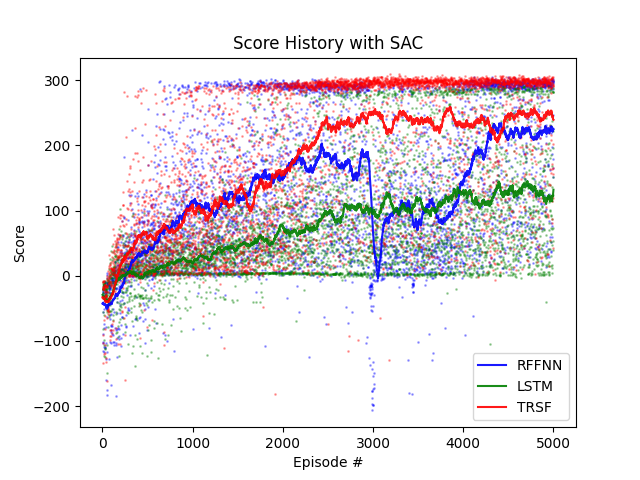
\includegraphics[width=0.95\textwidth]{figures/bipedal/SCATTER_SAC_RFFNN_LSTM_TRSF.png}
		\caption{SAC}
		\label{fig:sac_scatter_ep_rewards}
	\end{subfigure}
	\caption{Scatter Plot with Moving Average for Episode Scores}
\end{figure}

\begin{figure}[!ht]
	\centering
	\begin{subfigure}{.49\textwidth}
		\centering
		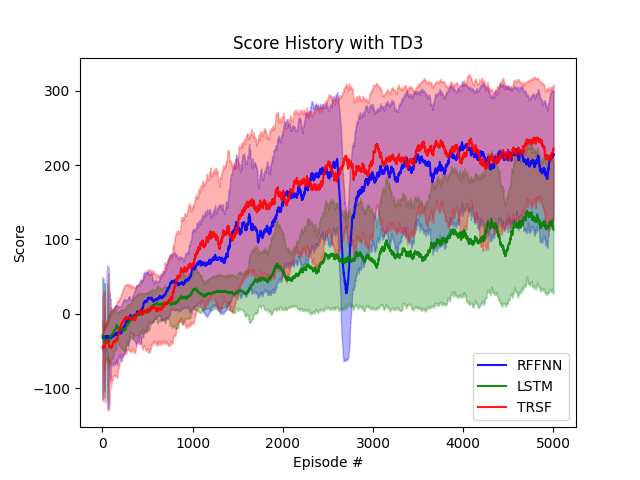
\includegraphics[width=0.99\textwidth]{figures/bipedal/STD_TD3_RFFNN_LSTM_TRSF.png}
		\caption{TD3}
		\label{fig:td3_std_ep_rewards}
	\end{subfigure}
	\begin{subfigure}{.49\textwidth}
		\centering
		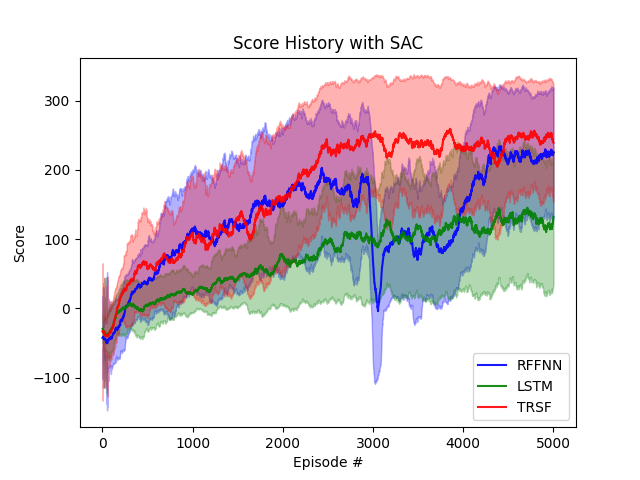
\includegraphics[width=0.95\textwidth]{figures/bipedal/STD_SAC_RFFNN_LSTM_TRSF.png}
		\caption{SAC}
		\label{fig:sac_std_ep_rewards}
	\end{subfigure}
	\caption{Moving Average and Standard Deviation for Episode Scores}
\end{figure}

Officially, 300 points in average required in random 100 simulations to say the environment is solved.
Therefore, none of our approaches solved.
However, they partially solved problems by exceeding 200 point limit, while some simulations yield around 280 points with all neural networks in TD3 and 300 points are reached with SAC. 

RFFNN seems to be enough for solving the problem, although there exist partial observability in the environment. 
That model reaches around 220 points in average with TD3 and 225 points with SAC. In addition, learning was unstable. 

The robot was able to walk by LSTM model but yield worse results and cannot exceed 120 points in average with both TD3 and SAC. 

Transformer model yield best results by reaching 230 points with TD3 and exceeds 250 points with SAC. 

As Transformer and RFFNN are relatively succesfull, their behavior is visualized in \figref{fig:rffnn_simulation} and \figref{fig:trsf_simulation} for TD3 model. 
The main behavioral difference is when the agent faces a big hurdle. 
First model passes it by jumping while other does by taking a very big step, shown in \figref{fig:anim_rffnn_hurdle} and \figref{fig:anim_trsf_hurdle}.

In SAC results, RFFNN and Transformer agents do not exhibit a noteworthy difference.

Also, SAC model performes better than TD3 in general. 
Agent cannot exceed 280 points in any simulation with TD3 (\figref{fig:td3_scatter_ep_rewards}) but it exceeds 300 points with SAC (\figref{fig:sac_scatter_ep_rewards}). Also, as seen from the moving average points, SAC agents are superior (\figref{fig:td3_std_ep_rewards},\figref{fig:sac_std_ep_rewards}).

\begin{figure}[!ht]
	\centering
	\begin{subfigure}{.9\textwidth}
		\centering
		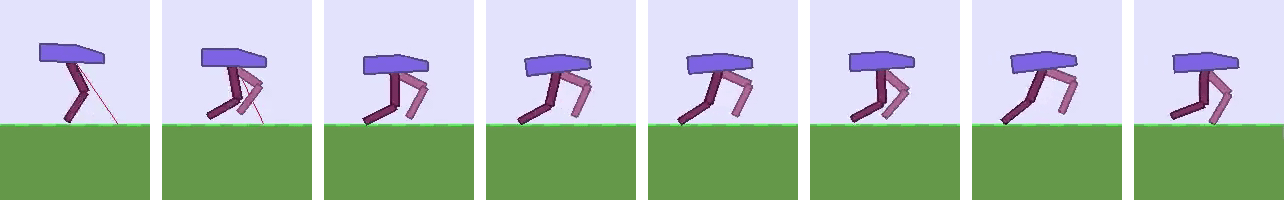
\includegraphics[width=0.99\textwidth]{figures/bipedal/anim/ff_flat.png}
		\caption{Flat Surface}
		\label{fig:anim_rffnn_flat}
	\end{subfigure}
	\begin{subfigure}{.9\textwidth}
		\centering
		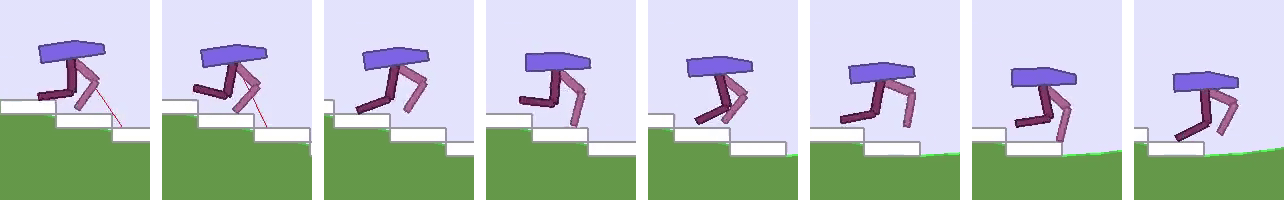
\includegraphics[width=0.99\textwidth]{figures/bipedal/anim/ff_stairs.png}
		\caption{Stairs}
		\label{fig:anim_rffnn_stairs}
	\end{subfigure}
	\begin{subfigure}{.9\textwidth}
		\centering
		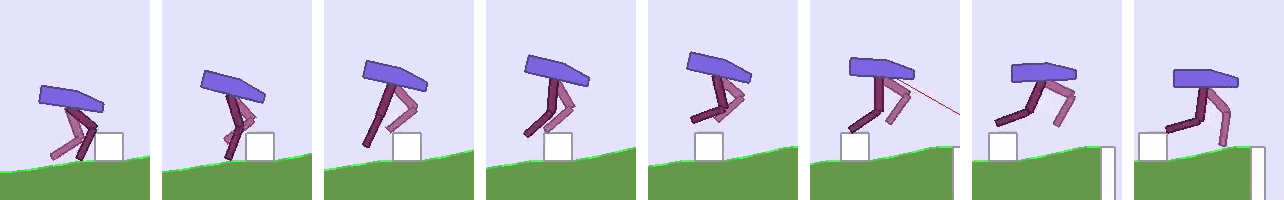
\includegraphics[width=0.99\textwidth]{figures/bipedal/anim/ff_hurdle.png}
		\caption{Hurdle}
		\label{fig:anim_rffnn_hurdle}
	\end{subfigure}
	\begin{subfigure}{.9\textwidth}
		\centering
		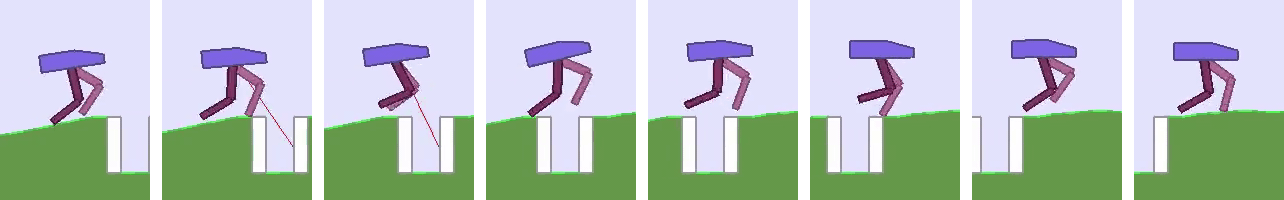
\includegraphics[width=0.99\textwidth]{figures/bipedal/anim/ff_pitfall.png}
		\caption{Pitfall}
		\label{fig:anim_rffnn_pitfall}
	\end{subfigure}
	\caption{Walking Simulation of RFFNN model at best version with TD3}
	\label{fig:rffnn_simulation}
\end{figure}

\begin{figure}[!ht]
	\centering
	\begin{subfigure}{.9\textwidth}
		\centering
		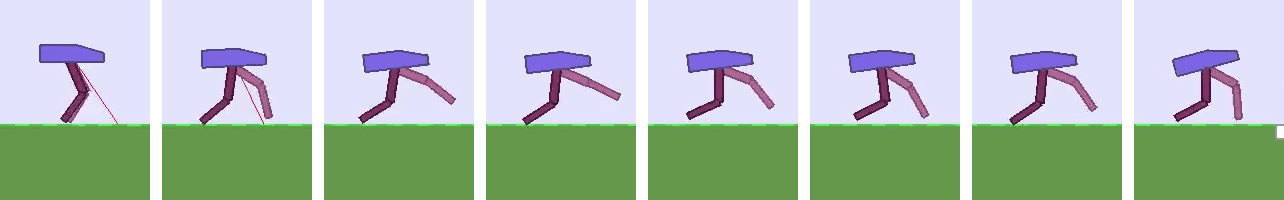
\includegraphics[width=0.99\textwidth]{figures/bipedal/anim/trsf_flat.png}
		\caption{Flat Surface}
		\label{fig:anim_trsf_flat}
	\end{subfigure}
	\begin{subfigure}{.9\textwidth}
		\centering
		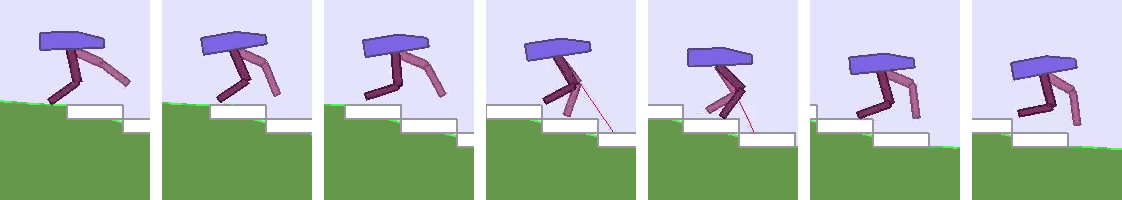
\includegraphics[width=0.99\textwidth]{figures/bipedal/anim/trsf_stairs.png}
		\caption{Stairs}
		\label{fig:anim_trsf_stairs}
	\end{subfigure}
	\begin{subfigure}{.9\textwidth}
		\centering
		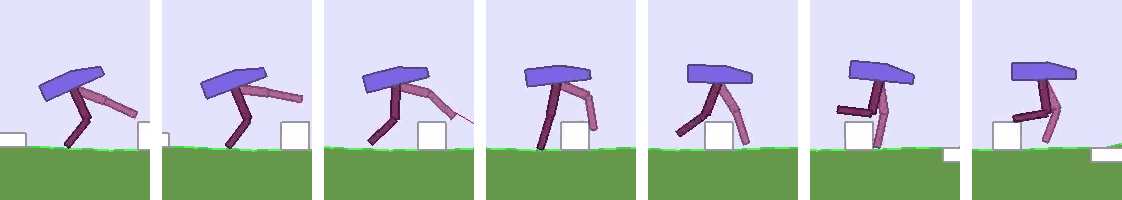
\includegraphics[width=0.99\textwidth]{figures/bipedal/anim/trsf_hurdle.png}
		\caption{Hurdle}
		\label{fig:anim_trsf_hurdle}
	\end{subfigure}
	\begin{subfigure}{.9\textwidth}
		\centering
		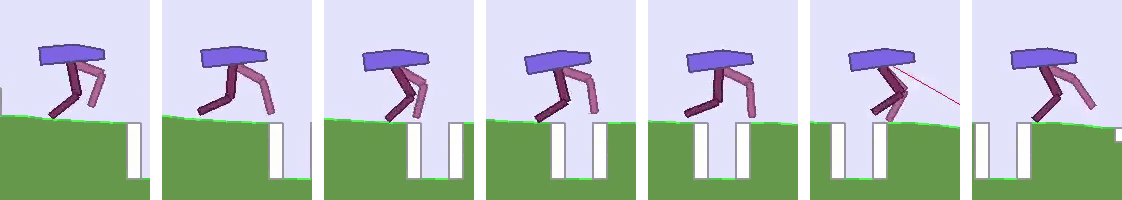
\includegraphics[width=0.99\textwidth]{figures/bipedal/anim/trsf_pitfall.png}
		\caption{Pitfall}
		\label{fig:anim_trsf_pitfall}
	\end{subfigure}
	\caption{Walking Simulation of Transformer model at best version with TD3}
	\label{fig:trsf_simulation}
\end{figure}
